\documentclass[12pt]{article}
\usepackage[margin=1 in]{geometry}
\usepackage{graphicx}
\usepackage{float}
\usepackage{booktabs}
\usepackage{siunitx}
\usepackage{amsmath}
\usepackage{amssymb}


\title{Lab 10: LTSpice Analysis of Active Filters}
\author{Sean Balbale}
\date{November 11th, 2024}
\setlength{\parindent}{0in}

\begin{document}

\begin{titlepage}
	\begin{center}
		\vspace*{1in}

		\Huge
		\textbf{Lab 10}

		\LARGE
		LTSpice Analysis of Active Filters

		\vspace{3 in}

		\textbf{Student Name:} Sean Balbale
		\\ \textbf{Instructor:} Dr. Iman Salama
		\\ \textbf{Lab Partner Name:} Krish Gupta
		\\ \textbf{Date:} November 15, 2024

		\vfill


	\end{center}
\end{titlepage}

\newpage

\section{Introduction}
Operational amplifiers (op-amps) have served as essential components in
electronic circuit design, particularly in sensing and signal processing
applications. This lab focused on constructing active filters with op-amps,
which are critical for biomedical applications such as electrocardiogram (EKG)
signal measurement. These filters were designed to amplify small signals while
selectively filtering out noise, thereby enhancing signal quality by rejecting
common-mode interference and removing unwanted frequency components. Through
LTSpice simulations, low-pass and high-pass filter designs were examined to
analyze their frequency responses, cutoff frequencies, and time-domain
performance. This approach provided insights into the role of active filters in
real-world signal processing, forming a foundation for practical applications in
biomedical and other electronic systems.



\section{Results}
% \begin{figure}[H]
% 	\centering
% 	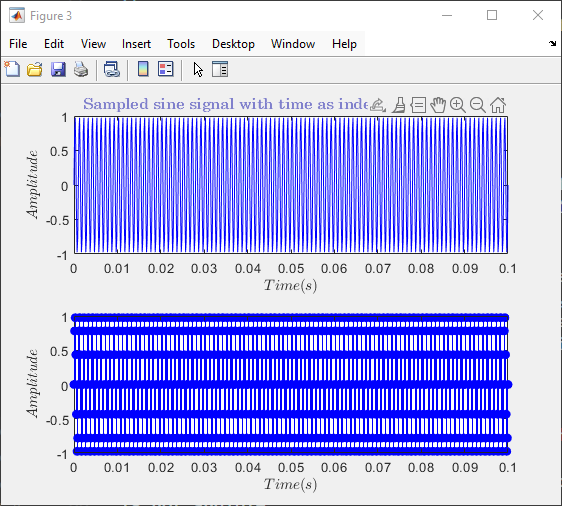
\includegraphics[width=0.3\textwidth]{fig 1f 7000.png}\hfill
% 	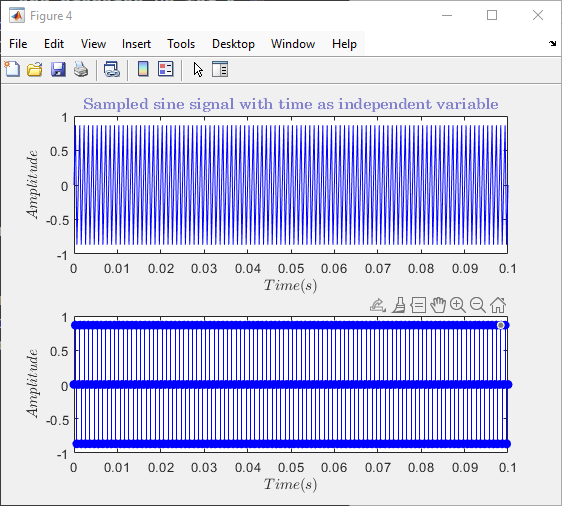
\includegraphics[width=0.3\textwidth]{fig 1f 3000.png}\hfill
% 	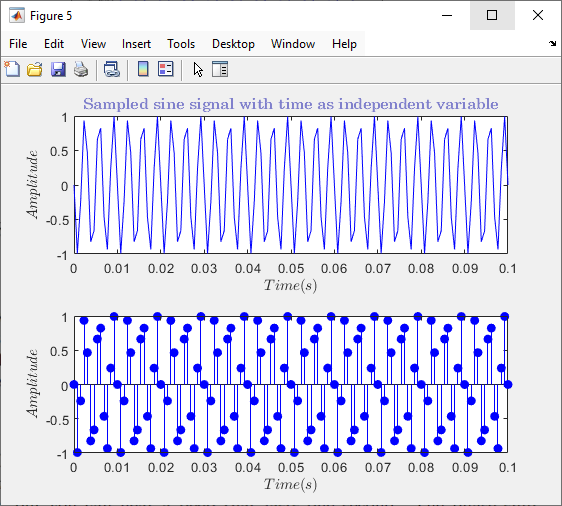
\includegraphics[width=0.3\textwidth]{fig 1f 1300.png}
% 	\caption{Sinusoidal with $f_s$ = 7 kHz, 3 kHz, and 1.3 kHz}
% 	\label{fig:fig3}
% % \end{figure}

\subsection{LTSpice Modeling of Op Amp Circuits}
\begin{figure}[H]
	\centering
	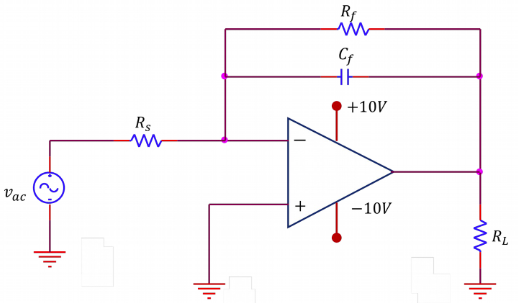
\includegraphics[width=0.5\textwidth]{photos/First Order Active Low Pass Filter.png}
	\caption{First Order Active Low Pass Filter}
	\label{fig:FirstOrderActiveLowPassFilter}
\end{figure}

A first order low pass filter was constructed using an op-amp, resistors
($R_f$, $R_s$, $R_L$), and capacitor ($C_f$). Following the circuit design
(Figure \ref{fig:FirstOrderActiveLowPassFilter}), the circuit was simulated in LTSpice
with $\pm \SI{10}{\volt} \; DC$ power supplies, $R_f = \SI{100}{\kilo\ohm}$, $R_s = \SI{20}{\kilo\ohm}$,
$R_L = \SI{1}{\kilo\ohm}$, and $C_f = \SI{10}{\nano\farad}$. The voltage input was a
AC input with a $\SI{0.1}{\volt}$ amplitude and a frequency sweep from $\SI{1}{\hertz}$
to $\SI{1}{\mega\hertz}$.
\newline

The frequency cutoff can be calculated using the formula:
\[
	\begin{aligned}
		f_c & = \frac{1}{2\pi R_f C_f}                                         \\
		    & = \frac{1}{2\pi \times 100 \times 10^3 \times 10 \times 10^{-9}} \\
			& = \SI{159.1}{\hertz}
	\end{aligned}
\]

This results in a cutoff frequency of $\SI{159.1}{\hertz}$.

This value is what is expected to be seen since there is a time constant of
$\SI{1}{\milli\second}$. Which was calculated using the formula:
\[
	\begin{aligned}
		\tau & = R_f \times C_f \\
		     & = 100 \times 10^3 \times 10 \times 10^{-9} \\
		     & = \SI{1}{\milli\second}
	\end{aligned}
\]
These theoretical values are confirmed by the LTSpice simulation results shown in Figure \ref{fig:1.2Results}.
\begin{figure}[H]
	\centering
	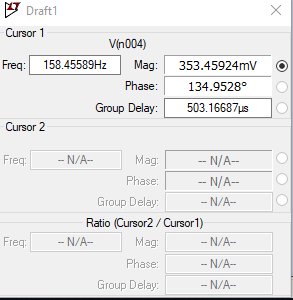
\includegraphics[width=0.5\textwidth]{Lab 10 Shared/1.2 simulation results.PNG}
	\caption{LTSpice Simulation Results}
	\label{fig:1.2Results}
\end{figure}

\begin{figure}[H]
	\centering
	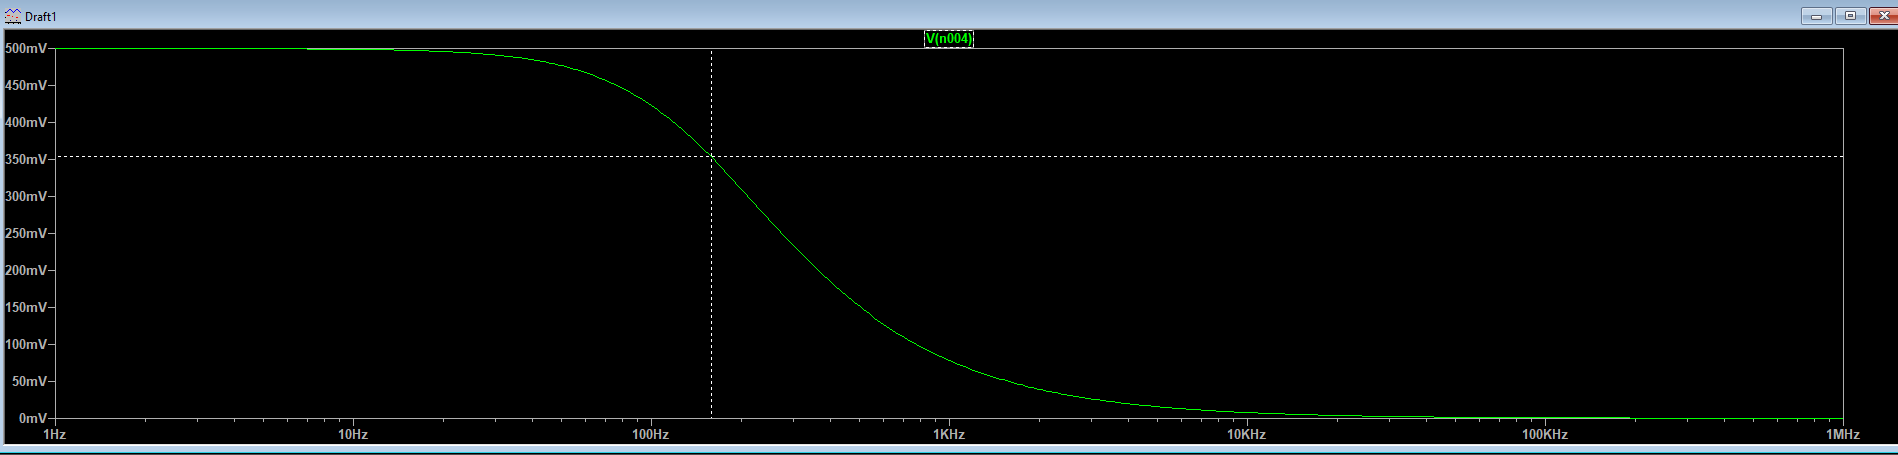
\includegraphics[width=1\textwidth]{Lab 10 Shared/1.2 simulation.PNG}
	\caption{LTSpice Simulation}
	\label{fig:1.2Simulation}
\end{figure}
These results can also be calculated by hand from Figure \ref{fig:1.2Simulation}.



\section{Discussion and Conclusion}


\section{References}
 [1] Dr. Iman Salama. “Lab 10 – LTSpice Analysis of Active Filters” Northeastern University. 11 November 2024.

\end{document}
